% !TeX spellcheck = en_US
\chapter{Deep Learning for CV}
\todo{}

\section{Image-to-Image Translation}
Image-to-image translation is a class of computer vision problems where the goal is to learn the mapping between an input image and an output image. It has various applications \cite{isola2017image, zhu2017unpaired}, \eg: 
\begin{itemize}
	\item Domain adaptation
	\item Semantic label $\leftrightarrow$ photo
	\item Map $\leftrightarrow$ aerial photo
	\item Edges $\rightarrow$ photo
	\item BW $\rightarrow$ color photos
	\item Day $\rightarrow$ night
	\item Photo with missing pixels $\rightarrow$ inpainted photo (recovering)
\end{itemize}
Recent approaches utilize \ac{GAN}.

\subsection{pix2pix}
\texttt{pix2pix} uses \ac{CGAN} idea with U-Net architecture \cite{isola2017image}.
\begin{figure}[hbt!]
	\centering
	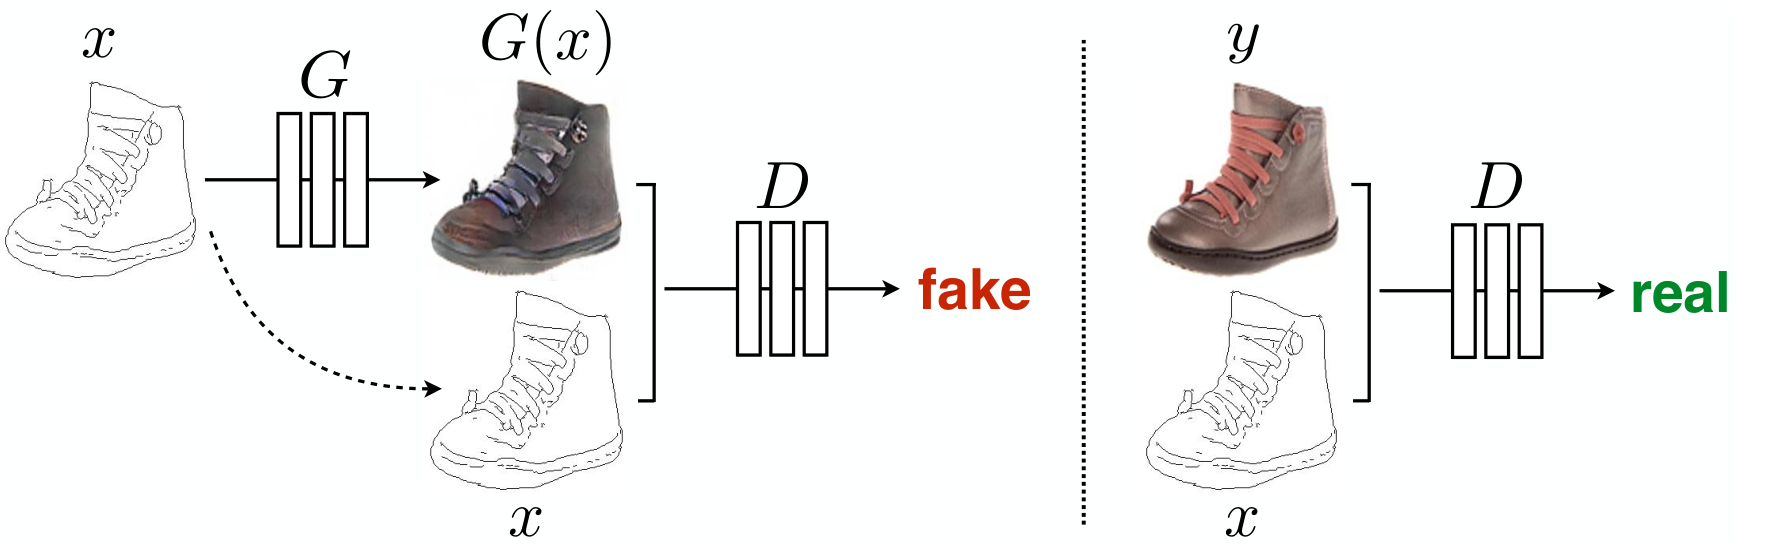
\includegraphics[width=0.9\textwidth]{pix2pix.png}
	\caption{Training a \ac{CGAN} to map edges $\rightarrow$ photo. Both the discriminator and generator are conditioned on the input $x$. \cite{isola2017image}}
\end{figure}

The loss function of \texttt{pix2pix} combines \ac{CGAN} objective with L1 distance with ground-truth images. L1 distance is prefer over L2 because L1 encourage less blurring effect.
\begin{align}
	\mathcal{L}_{GAN}(G,D) &= \mathbb{E}_y [\log D(y)] + \mathbb{E}_z [\log (1-D(G(z)))]\\
	\mathcal{L}_{CGAN}(G,D) &= \mathbb{E}_{x,y} [\log D(x,y)] + \mathbb{E}_{x,z} [\log (1-D(x,G(x,z)))]\\
	\mathcal{L}_{L1}(G) &= \mathbb{E}_{x,y,z} \big[ ||y-G(x,z)||_1 \big]\\
	G* &= \arg \underset{G}{\min} \underset{D}{\max} \mathcal{L}_{CGAN}(G,D) + \lambda \mathcal{L}_{L1}(G)
\end{align}

\note In implementation, the noise $z$ is accounted as DropOut percentage.

\subsection{CycleGAN}
Cycle\ac{GAN} addresses the problem when there is no \hlb{available paired training data}. By considering cycle consistency losses, it limits the mapping functions. \cite{zhu2017unpaired}
\begin{align}
	&G: X \rightarrow Y &&-\text{mapping from domain $X$ to domain $Y$}\\
	&F: Y \rightarrow X &&-\text{mapping from domain $Y$ to domain $X$}\\
	&F(G(x)) \approx x &&-\text{forward cycle consistency}\\
	&G(F(y)) \approx y &&-\text{backward cycle consistency}
\end{align}
\begin{align}
	\mathcal{L}_{GAN_1} (G, D_Y, X, Y) &= \mathbb{E}_{y \sim p_{data}(y)}[\log D_Y(y)] + \mathbb{E}_{x \sim p_{data}(x)} [\log (1 - D_Y(G(x)))]\\
	\mathcal{L}_{GAN_2} (F, D_X, X, Y) &= \mathbb{E}_{x \sim p_{data}(x)}[\log D_X(x)] + \mathbb{E}_{y \sim p_{data}(y)} [\log (1 - D_X(F(y)))]\\
	\mathcal{L}_{cyc}(G,F) &= \mathbb{E}_{x \sim p_{data}(x)}\big[||F(G(x))-x||_1 \big] + \mathbb{E}_{y \sim p_{data}(y)} \big[||G(F(y))-y||_1\big]\\
	\mathcal{L}(G, F, D_X, D_Y) &= \mathcal{L}_{GAN_1} (G, D_Y, X, Y) + \mathcal{L}_{GAN_2} (F, D_X, X, Y) + \lambda \mathcal{L}_{cyc}(G,F)\\
	G^*, F^* &= \arg\underset{G, F}{\min}\underset{D_X, D_Y}{\max} \mathcal{L}(G, F, D_X, D_Y)
\end{align}
\begin{figure}[hbt!]
	\centering
	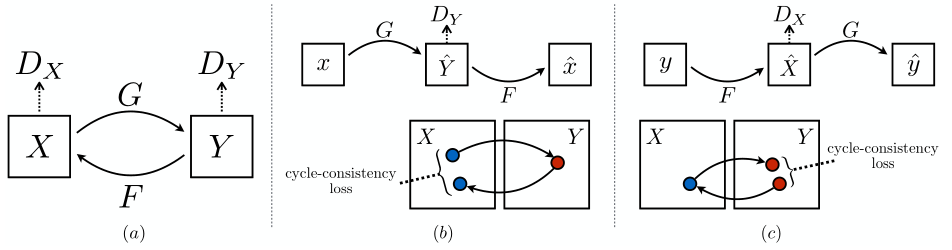
\includegraphics[width=\textwidth]{cyclegan.png}
	\caption{Cycle\ac{GAN} structure with 4 networks. \cite{zhu2017unpaired}}
\end{figure}

\note
\begin{itemize}
	\item The authors mention that experiment the cycle consistency loss as adversarial loss leads to no improved performance.
	\item Cycle\ac{GAN}'s results are not significantly better than pix2pix's.
	\item Perform well on tasks relating color transformation (\eg style transfer: picture $\leftrightarrow$ paintings, horse $\leftrightarrow$ zebra, winter $\leftrightarrow$ summer), but not so good with \hlb{geometric changes} (dog $\leftrightarrow$ cat).
\end{itemize}
